\documentclass{article}
\usepackage[utf8]{inputenc}
\usepackage[options ]{algorithm2e}
\usepackage{algorithmic}
\usepackage{algorithm}
\usepackage{graphicx}
\graphicspath{ {./images/} }
\usepackage[english]{babel}
\usepackage[utf8]{inputenc}
\usepackage{amsmath}
\usepackage{amsfonts}
\usepackage{graphicx}
\usepackage[colorinlistoftodos]{todonotes}
\usepackage{algorithm}
\usepackage{algpseudocode}

\title{Critical Sections Lab Assignment}
\author{Diaconescu Bogdan-Florin\\ CR 3.2 A, Anul 3}
\date{November 2019}

\begin{document}

\maketitle

\section{Problem statement}
\hspace{0.5 cm}
    Trebuie sa implementam in Promela un algoritm pentru numararea concurenta si sa analizam ce valoare poate lua n la sfarsitul executiei programului.
    
\section{Implementation/Solution}
\hspace{0.5 cm}
Am folosit un MACRO TIMES 10 deoarece doresc ca fiecare proces sa incrementeze variabila n de 10 ori. Am definit 2 variabile "n" si "finished" de tipul byte, echivalent cu uchar in C, ce pot lua valori cuprinde intre 1 si 255. Variabila n este cea care trebuie incrementata, iar variabila finished este folosita pentru a marca terminarea procesului(cand se termina un proces variabila finished se incrementeaza). Acestea sunt variabile globale ce pot fi utilizate in toate procesele.

\hspace{0.5 cm}
La linia 5 am creat 2 procese P in interiorul carora am declarat 2 variabile de tipul byte "i" si "temp" utilizate la incrementarea numarului n.  La linia 8 am folosit o bucla "do" urmata de 2 conditii. Daca i este mai mare decat TIMES inseamna ca numarul s-a incrementat deja de 10 ori si se iese din bucla. In caz contrat, se efectueaza incrementarea numarului. Dupa iesirea din bucla se incrementeaza si variabila finished.

\hspace{0.5 cm}
La linia 17 am creat un nou proces numit "main". In acesta se verifica daca finished are valoarea 2, adica daca cele 2 procese s-au incheiat. In caz contrar, se asteapta terminarea acestora. Apoi se afiseaza valoarea finala a lui n.

\section{Experimental data}
\hspace{0.5 cm}
Am rulat algoritmul de mai multe ori folosind optiunea Random. De fiecare data la iesire n avea valori apropiate de 20, dar niciodata valoarea 20. Se observa ca valoarea finala a variabilei finished este 2, ceea ce inseamna ca ambele procese s-au incheiat.

\hspace{0.5 cm}
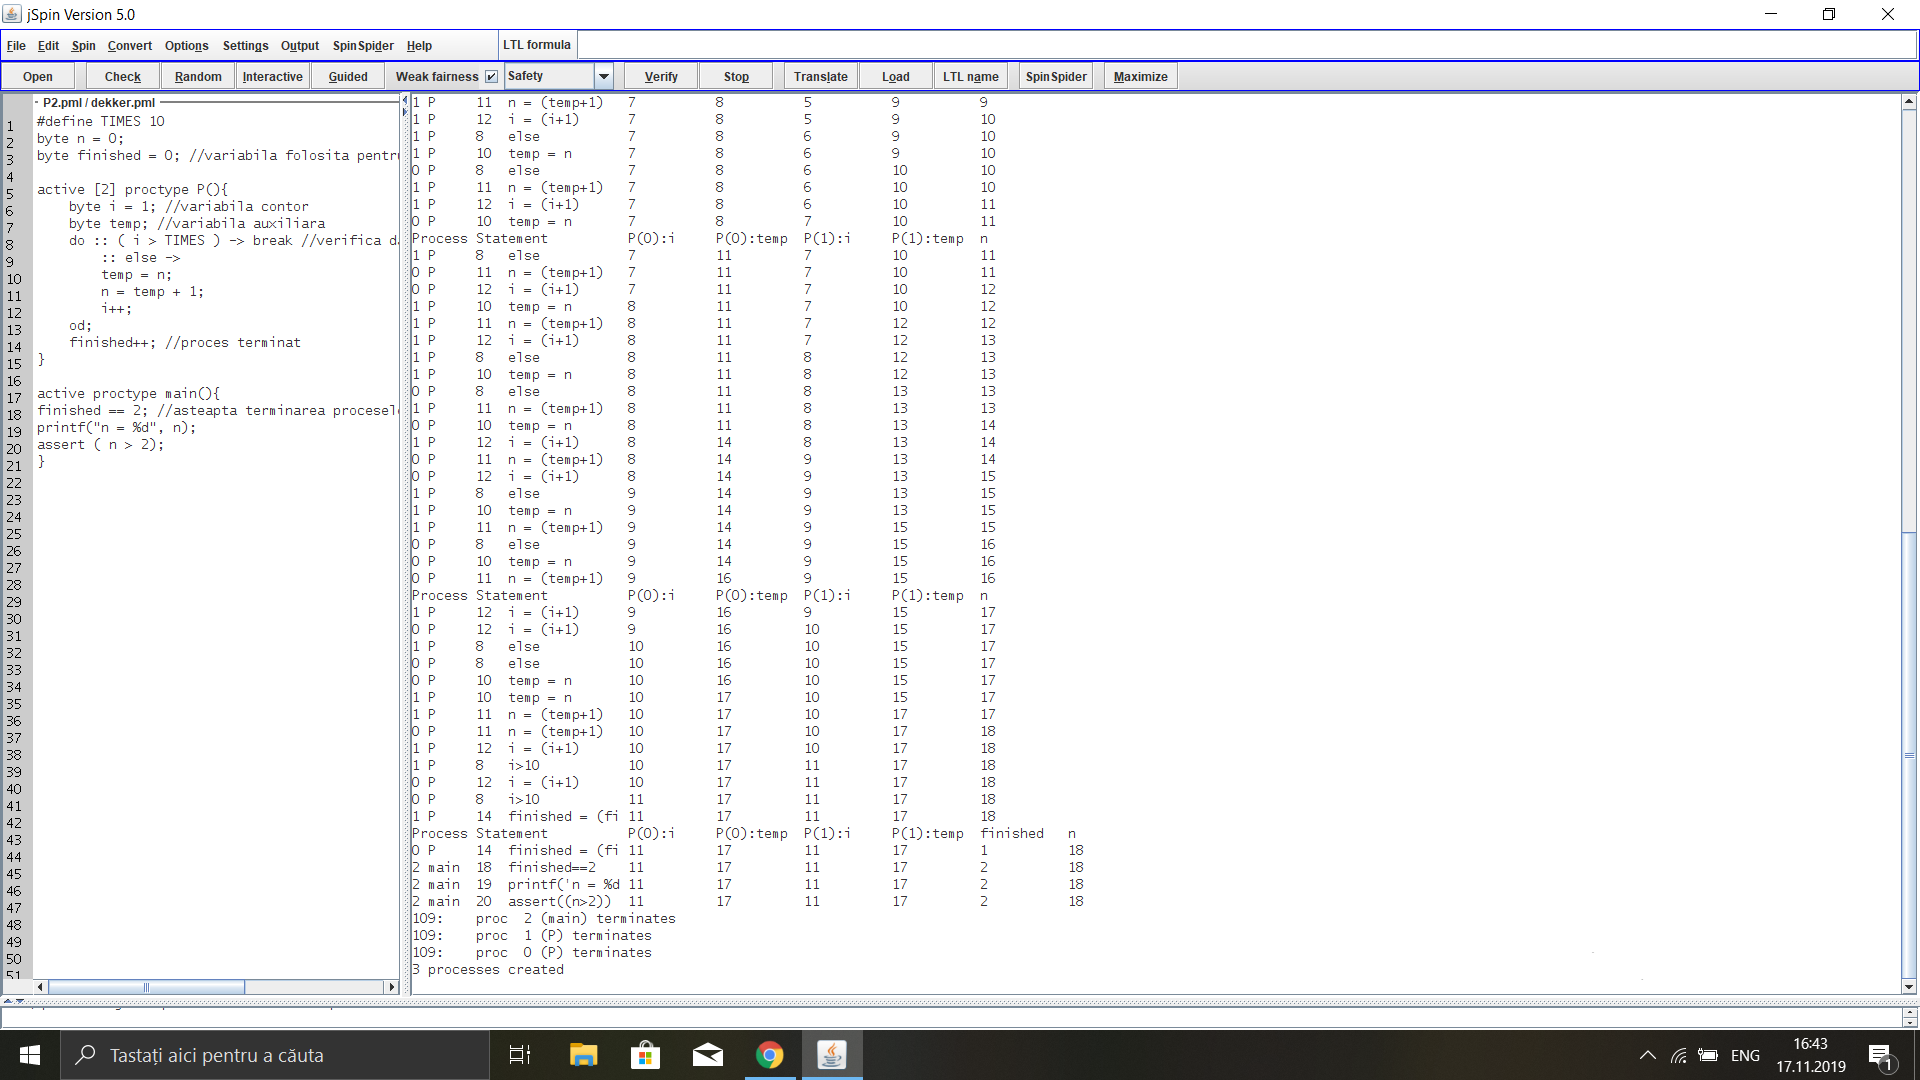
\includegraphics[width=2.2\textwidth]{P2_1.png}
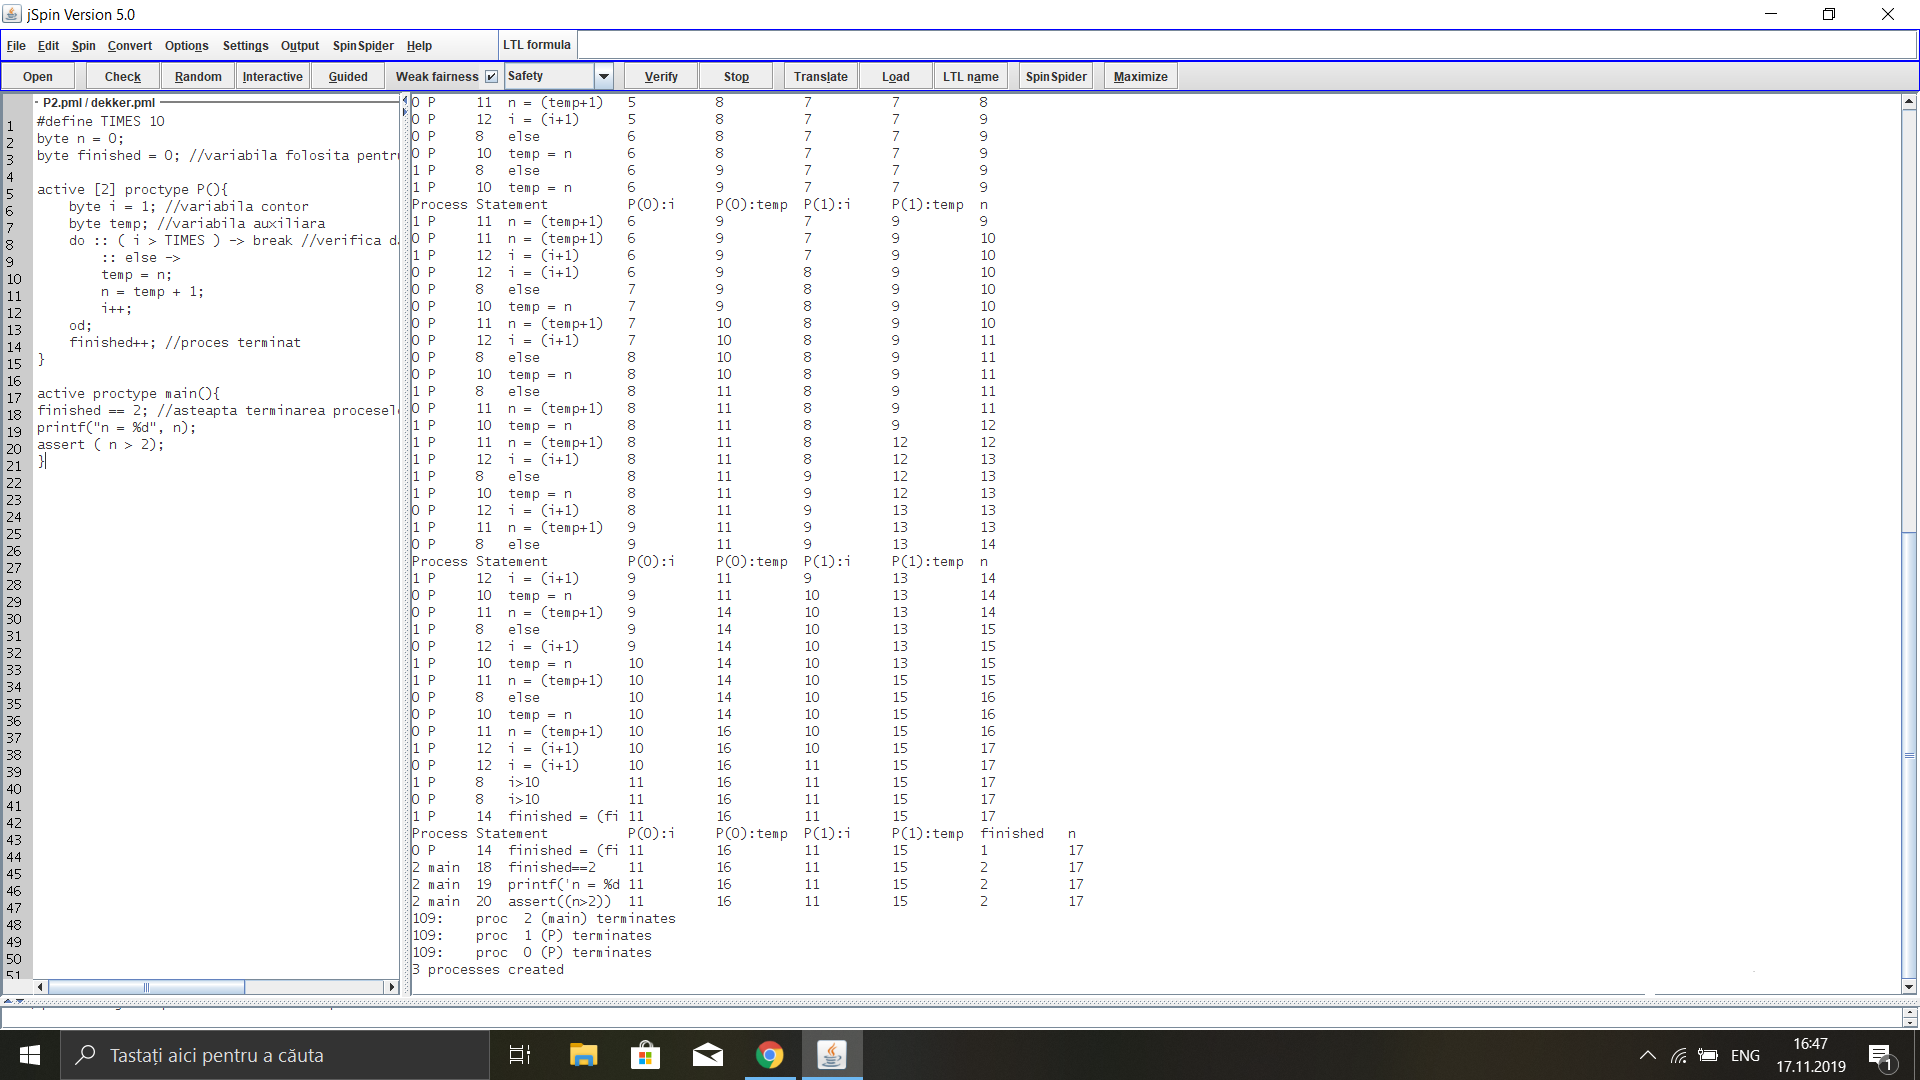
\includegraphics[width=2.2\textwidth]{images/P2_2.png}
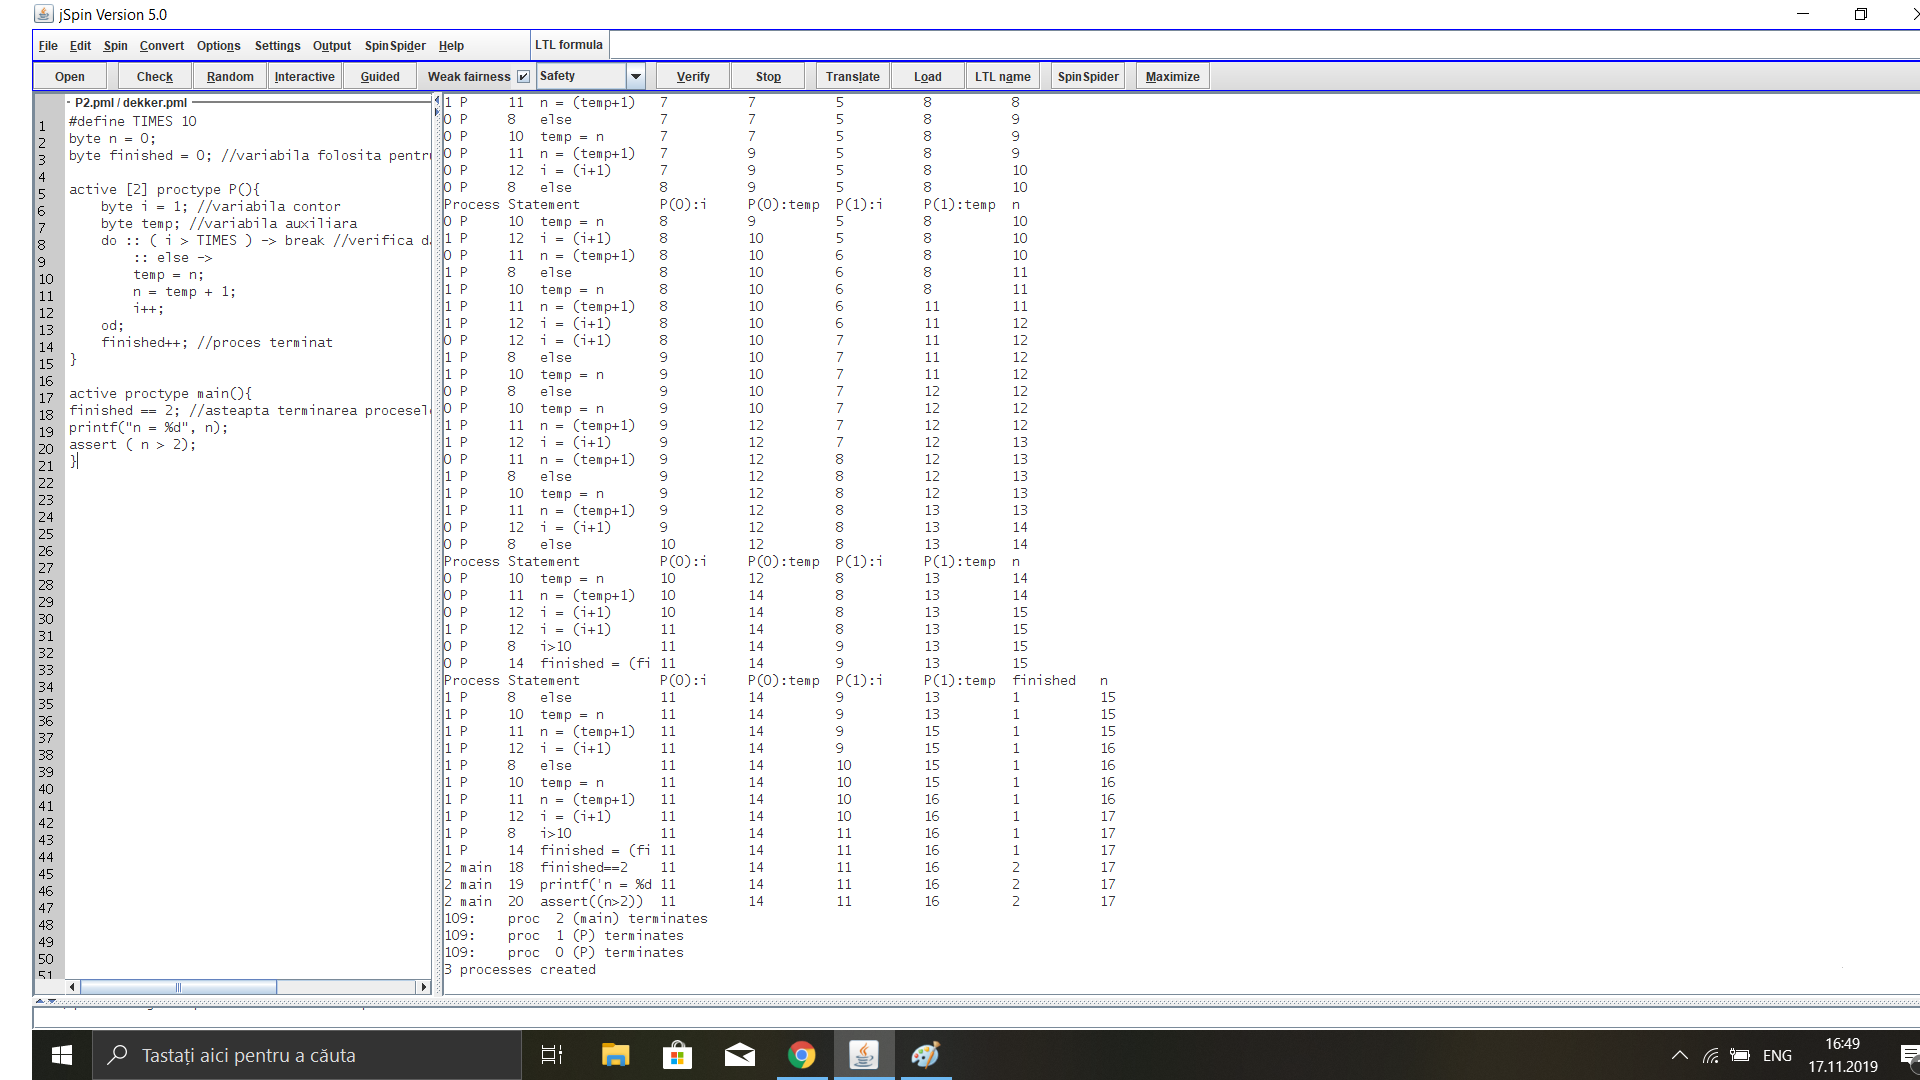
\includegraphics[width=2.2\textwidth]{images/P2_3.png}

\section{Results \& Conclusions}
\hspace{0.5 cm}
Am implementat in Promela numararea concurenta utilizand o variabila n si 2 procese care incrementeaza fiecare variabila n de 10 ori. Am implementat instructiunea "for" utilizand bucla "do" si explicand ce trebuie sa faca algoritmul in cazul in care o conditie nu este indeplinita. Valoarea finala a lui n a fost apropiata de 20, dar niciodata 20, desi am rulat programul de mai multe ori pentru a-l testa.


\end{document}
